\section{SpatialNet}\label{sec:method}

\subsection{Task}\label{sec:task}
Given one RGB frame from a head-worn camera, SpatialNet predicts the box $\bH$ of the wearer's hand, the fingertip $\tip$, the pointing direction $\dir$ in the image plane and the box $\bT$ of the pointed-at object, which we call the \emph{target}. It also predicts three presence flags: the wearer's hand is visible, the hand is pointing, and something is pointed at. Boxes and points are normalised to $[0,1]$. Two requirements separate the task from generic detection. \emph{Ownership}: when several hands are visible, all outputs must refer to the wearer's hand, and a frame showing only other people's hands has no wearer's hand. \emph{Budget}: the model must run on the glasses' own processor, without a second network or a server call, within the 100--200\,ms commonly targeted for interactive response~\cite{miller1968response,card1991information}. We do not recognise \emph{what} the target is. $\bT$ is the region that a later step, such as an object recogniser or a visual question-answering model, takes as input, so that this step can run on a small crop and only when the wearer points; Section~\ref{sec:choice} tests such a recogniser.

\subsection{Architecture}\label{sec:arch}
Figure~\ref{fig:arch} shows the network. A shared trunk turns the frame into one feature map. Four heads then run in a fixed order (wearer's hand, fingertip, pointing direction, target), and each head reads the shared map \emph{at the location that the previous head predicted}: the fingertip is searched for around the hand that was found, the direction is computed from features of that hand and fingertip, and the target is searched for along the resulting ray. We call these heads \emph{instance-anchored}. Everything runs in a single forward pass, with no external hand detector, no language input and no hand box at test time.

\begin{figure}[t]
  \centering
  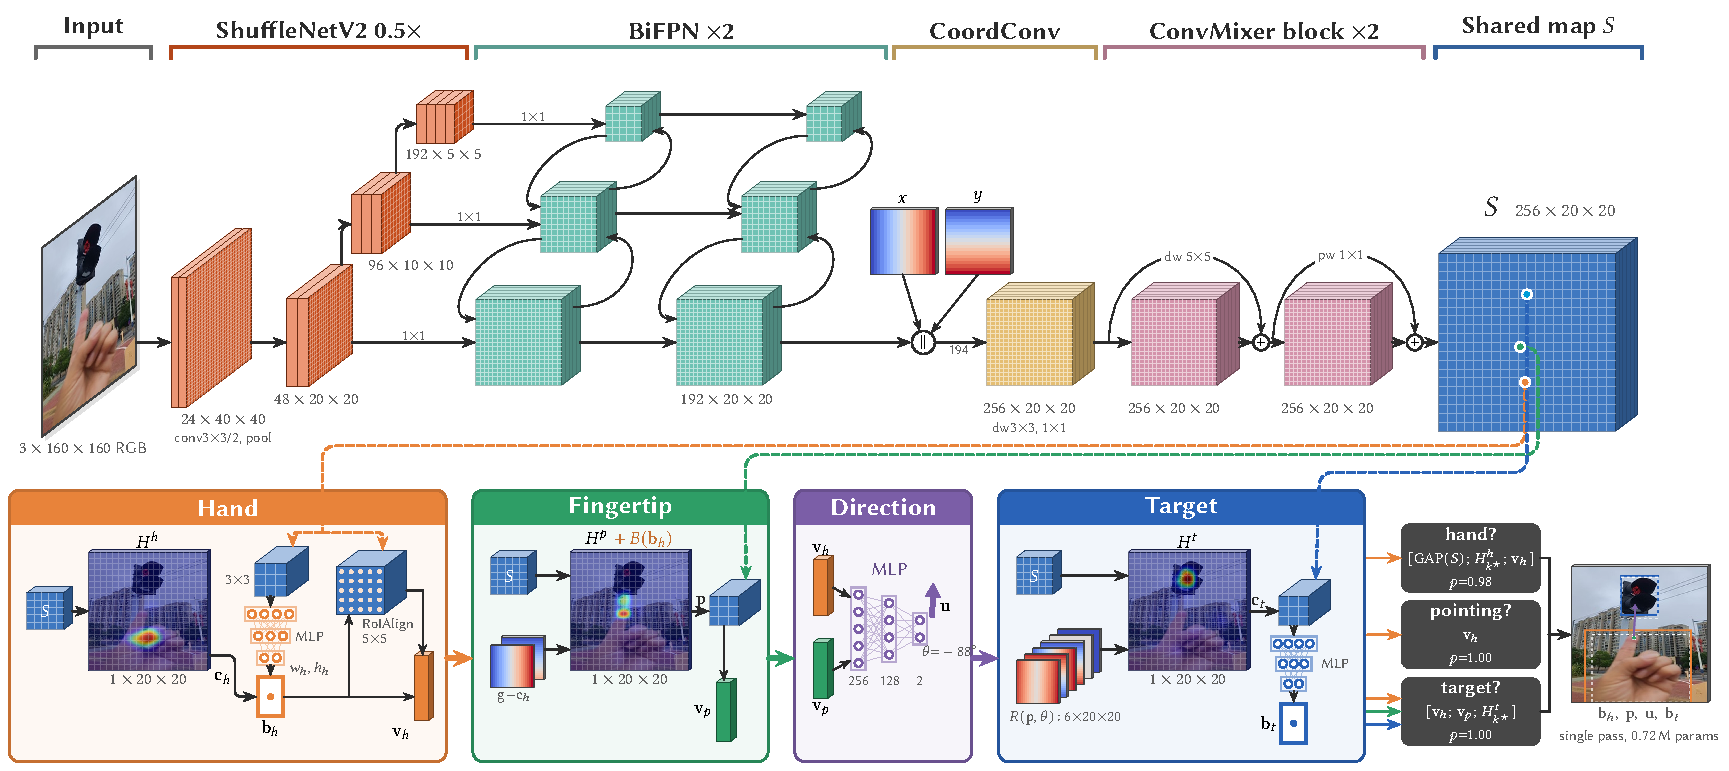
\includegraphics[width=\textwidth]{figures/architecture}
  \caption{SpatialNet. The trunk (top) turns one $160\times160$ frame into the shared map $S$ ($256\times20\times20$). Four heads (middle) run in order; dashed lines mark where a head samples $S$ at the location the previous head predicted: the hand centre $\cH$, the fingertip $\tip$ and the target centre $\cT$. Right: the presence gates and the decoded output. Heatmaps, ray-coordinate maps, gate probabilities and the output are real outputs of the trained model on one test image; each heatmap is overlaid on the input frame.}
  \Description{Block diagram drawn as three-dimensional tensor slabs. The input frame passes through a ShuffleNetV2 backbone whose three scales feed two BiFPN layers; the 20x20 output gets two coordinate channels, is reduced to 256 channels and passes two ConvMixer blocks to give the shared map S. Four coloured panels show the heads in sequence: wearer hand, fingertip, pointing direction and pointed target. Dashed lines from S show where each head samples it. On the right, three presence gates list their inputs and probabilities, and the output frame shows the predicted hand box, fingertip, direction and target box.}
  \label{fig:arch}
\end{figure}

\paragraph{Trunk.} The frame is resized to $160\times160$. A ShuffleNetV2~0.5$\times$ backbone~\cite{ma2018shufflenet}, pretrained on ImageNet~\cite{deng2009imagenet}, feeds two BiFPN layers~\cite{tan2020efficientdet}, coordinate channels~\cite{liu2018coordconv} and two ConvMixer-style blocks~\cite{trockman2023patches}, which give the shared map $S$. Each head predicts a $20\times20$ heatmap and turns it into a point with a soft-argmax~\cite{sun2018integral} restricted to a small window around the peak, so that the estimate follows one instance even when two hands are visible (Appendix~\ref{app:method}).

\paragraph{Heads.} The \emph{hand} head predicts the hand centre; a $3\times3$ sample of $S$ around it gives the box size, and a RoIAlign-style sample over the box~\cite{he2017mask} gives a descriptor $\vH$ of this hand. The \emph{fingertip} heatmap adds two terms to the visual evidence: a learned term over each cell's offset from the hand centre, and a fixed prior that is zero inside the slightly enlarged hand box and falls outside it, which rules out the fingertips of other hands. A sample around the fingertip gives a descriptor $\vP$. The \emph{direction} head, an MLP on $[\vH;\vP]$, outputs a unit vector $\dir$ in the image plane; it is supervised with the direction from the labelled fingertip to the labelled target centre, so it is the direction \emph{to the target} as seen in the image. The \emph{target} head receives, for every cell, its position relative to the predicted ray: the offset from the fingertip, the distance along the ray and from its line, and the direction itself. A small branch, initialised at zero, turns these ray coordinates into a learned multiplicative prior on the visual evidence, so the network uses the ray only as far as it lowers the loss. The target box then follows as for the hand. Three MLP \emph{gates} decide whether the wearer's hand is present, whether it points and whether something is pointed at. The pointing and target gates read instance descriptors, so that another person's hand elsewhere in the frame does not switch them on by itself. The network has 722,104 parameters and costs 0.231 GFLOPs per frame, and its FP16 weights take 1.6\,MB (Table~\ref{tab:params}).

\subsection{Learning Whose Hand It Is}\label{sec:ownership}
No public pointing dataset labels other people's hands, and EgoPoint frames contain only the wearer's. We therefore paste hands into the frames during training (Figure~\ref{fig:ownership}). The procedure follows copy-paste augmentation~\cite{dwibedi2017cut,ghiasi2021simple}, but with the opposite aim: pasted hands are \emph{not} labelled, and the model is penalised for responding to them. One or two hand crops from other training images are pasted into half of the images with a hand and 30\% of those without, mostly rotated and placed in the upper part of the frame, away from the wearer's hand and the target. In 30\% of cases the pasted crop is the wearer's own hand, so that appearance alone cannot tell the two apart and the model has to use position, orientation and context. Labels never change: a no-hand image with a pasted hand stays \emph{no hand}, which teaches the hand gate to answer for the wearer only, and in the hand-heatmap loss a response near a pasted hand costs up to five times as much as one on background. The procedure encodes a prior: the wearer's arm enters from the bottom of the frame, while other people's hands appear higher and in other orientations. This holds for most use of glasses but can fail, for example when a companion's hand is near the bottom of the view (Section~\ref{sec:discussion}). Appendix~\ref{app:aug} lists all settings.

\begin{figure}[t]
  \centering
  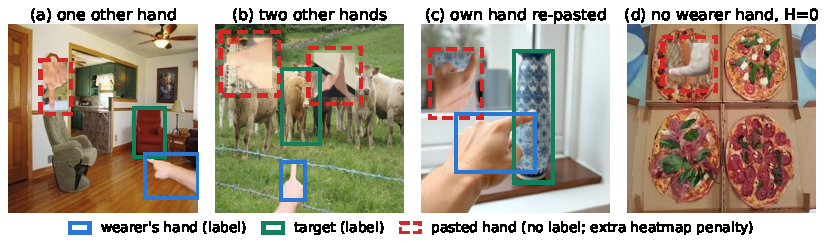
\includegraphics[width=\linewidth]{figures/ownership_examples}
  \caption{Distractor-hand pasting, produced by the training code. Pasted hands (red, dashed) come from other images (a, b) or from the same image (c), are rotated so that they rarely enter from the bottom edge, and are never labelled. A no-hand image with a pasted hand keeps the label \emph{no hand} (d).}
  \Description{Four training images. In the first two, one or two hands cut from other photos are pasted into the upper part of the image, rotated, and marked with red dashed boxes, while the wearer's pointing hand and the target keep their blue and green label boxes. In the third, a rotated copy of the wearer's own hand is pasted in the upper left. In the fourth, a pizza photo without a wearer's hand receives a pasted hand and keeps the label no hand.}
  \label{fig:ownership}
\end{figure}

\subsection{Training}\label{sec:training}
The loss sums 13 terms: box losses for the hand and the target, a keypoint loss for the fingertip, a cosine loss for the direction, focal heatmap losses at the hand centre, fingertip and target centre, focal losses for the gates, and two consistency terms that use predictions only (the predicted target should lie on the predicted ray, and the direction should roughly follow the hand-to-fingertip axis). Early in training, ground-truth anchors replace the predicted ones with a probability that decays to zero over 20 epochs, so that the downstream heads do not learn from meaningless locations. Appendix~\ref{app:method} gives the equations, the loss weights (Table~\ref{tab:weights}) and the training schedule.
